% main.tex
\documentclass[12pt, twoside]{book}

%%%%%%%% Preamble %%%%%%%%%%%%
\title{Guía de Armado de Telescopios}
\usepackage[utf8]{inputenc}
\usepackage[greek, spanish, es-noindentfirst, es-nolists, es-noshorthands]{babel}
\usepackage{amsmath}
\usepackage{amssymb}
\usepackage{graphicx}
\usepackage{xcolor}
\usepackage{float}
\usepackage{capt-of}
\usepackage{sidecap}
\usepackage{caption}
\usepackage{commath}
\usepackage{cancel}
\usepackage{anysize}
\usepackage{appendix}
\usepackage{tocbibind}
\usepackage{anyfontsize}
\usepackage{fancyhdr}
\usepackage{hyperref}
\usepackage{geometry}
\usepackage{booktabs}
\usepackage[backend=biber, style=ieee]{biblatex} % Usa Biber como backend
\usepackage[most]{tcolorbox}


% Configuración de rutas
\graphicspath{{./images/}}
\addbibresource{bib/references.bib}

% Configuración de página
\geometry{
	left=2.5cm,
	right=2.5cm,
	top=2.5cm,
	bottom=2.5cm
}

% Configuracion de Encabezado
% En el preámbulo (después de cargar los paquetes)
\usepackage{tikz} % Para elementos gráficos
\usetikzlibrary{positioning}

% Configuración avanzada del encabezado
\renewcommand{\headrule}{%
	\color{blue!60!black}\hrule width\textwidth height 1.2pt \vspace{1pt}%
	\color{blue!40!black}\hrule width\textwidth height 0.4pt%
}

\fancyhead[LE,RO]{%
	\begin{tikzpicture}[remember picture,overlay]
		\node[anchor=north west] at (current page.north west) {%
			\includegraphics[height=1.2cm]{images/logo-escuela}%
		};
		\node[anchor=north east] at (current page.north east) {%
			\textcolor{blue!80!black}{\footnotesize Página \thepage}%
		};
	\end{tikzpicture}%
}

\fancyhead[RE,LO]{\textcolor{blue!80!black}{%
		\footnotesize Guía de Armado de Telescopios | \leftmark%
}}

% Estilos de títulos
\newcommand\mymaintitlesize{\fontsize{16pt}{19.2pt}\selectfont}
\newcommand\mysubtitlesize{\fontsize{14pt}{16.8pt}\selectfont}

% Configuración de encabezados y pies de página
\pagestyle{fancy}


\fancyhf{}
\fancyhead[LE,RO]{\footnotesize Guía de Armado de Telescopios}
\fancyhead[RE,LO]{\footnotesize Optica Chapter - YT}
\fancyfoot[C]{\thepage}
\renewcommand{\footrulewidth}{0.4pt}

% Entorno	s matemáticos (opcional)
\newtheorem{definicion}{Definición}
\newtheorem{ejemplo}{Ejemplo}
\newtheorem{consejo}{Consejo Práctico}

% Renombrado de tablas
\addto\captionsspanish{% 
	\renewcommand{\listtablename}{Índice de tablas} % Cambia el título
}

% Crear un contador para numerar las cajas
\newtcolorbox[auto counter, number within=section]{pabox}[2][]{%
	colback=red!5!white,
	colframe=red!75!black,
	fonttitle=\bfseries,
	title=Definición~\thetcbcounter: #2,
	#1
}

% Crear una nueva caja basada en el contador anterior
\NewTColorBox[use counter from=pabox]{mybox}{ O{red} m d"" !O{} }{%
	enhanced,
	colframe=#1!75!black,
	colback=#1!5!white,
	fonttitle=\bfseries,
	title={\thetcbcounter~#2},
	IfValueT={#3}{watermark text={#3}},
	#4
}
%%%%%%%% Preamble ends %%%%%%%%%%%%

\begin{document}
	
	%%%%%%%%%%%%%%%%%%%%%%%%%%%%%%%% Portada %%%%%%%%%%%%%%%%%%%%%%%%%%%%%%%%%%
	\thispagestyle{empty}
	\begin{center}
		\begin{figure}[h]
			\centering
			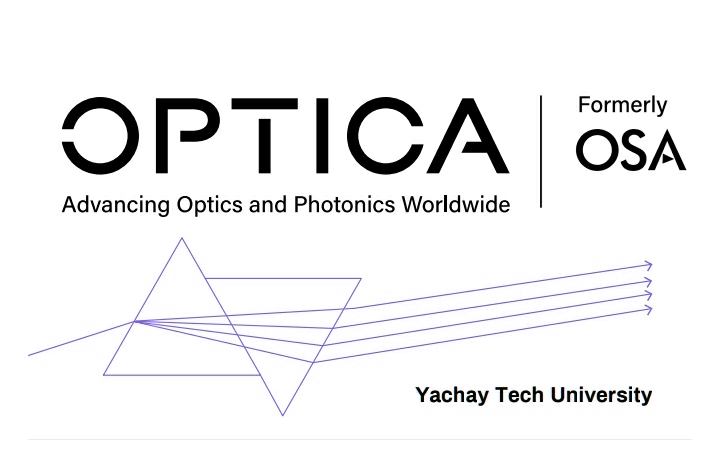
\includegraphics[width=0.7\textwidth]{logo_invertido}
		\end{figure}
		\vspace*{1cm}
		
		{\mymaintitlesize\textbf{Guía Práctica de Armado de Telescopios}}\\
		\vspace{1cm}
		{\mysubtitlesize\textbf{Curso de Óptica Experimental y Técnicas de Observación}}\\
		\vspace{2cm}
		{\mysubtitlesize\textbf{Instructor:}\\
			Damian Andrango - Físico\\
			\vspace{1cm}
			\textbf{Edición:}\\
			Abril 2024\\
			\vspace{1cm}
			\textbf{Duración del curso:}\\
			20 horas teórico-prácticas}
	\end{center}
	\clearpage
	
	%%%%%%%%%%%%%%%%%%%% Front Matter %%%%%%%%%%%%%%%%%%%%%%%%%
	\frontmatter
	
	\tableofcontents
	\cleardoublepage
%	\listoffigures
%	\listoftables
	
	\mainmatter
	
	%%%%%%%%%%%%%%%%%%%% Módulos Principales %%%%%%%%%%%%%%%%%%%%%%%%%
	
	Este documento es una guía teórico-práctica que acompañará el desarrollo del curso de construcción de telescopios ópticos de bajo costo, utilizando herramientas digitales como impresión 3D, diseño CAD y corte láser.
	
	La iniciativa nace desde el grupo del Capítulo de Óptica, con el propósito de diseñar y fabricar telescopios accesibles que puedan ser llevados a escuelas, acercando la astronomía a comunidades con recursos limitados. A lo largo del curso, no solo aprenderemos cómo funcionan los telescopios, sino que también construiremos uno funcional desde cero.
	
	Cada módulo está diseñado para ser abordado en sesiones de 2 a 2,5 horas, divididas en bloques de trabajo (pomodoros). Al finalizar, cada participante contará con un prototipo propio, adaptado a sus ideas y preferencias. También se introducirán habilidades prácticas como modelado 3D en SolidWorks, preparación de piezas con slicers para impresión 3D, y diseño de planos para corte láser.
	
	Como punto de partida, utilizaremos un prototipo inicial ya empezado, el cual servirá de referencia tanto para el aprendizaje como para su presentación ante potenciales inversionistas, con miras a escalar el proyecto.
	
	Cabe señalar que para llevar a cabo la construcción de los telescopios será necesario adquirir ciertos materiales y componentes clave, como espejos y oculares, filamento para impresión 3D, tubos de PVC, maderas para las bases, entre otros. Estos elementos serán definidos y organizados durante las primeras sesiones del curso, priorizando soluciones de bajo costo y materiales disponibles localmente o por compra con envío en corto tiempo. internacional. 
	
	
	\chapter{Telescopios Generalidades}
	\label{telescopes_general}
	% Modulo 1: Telescopios-Generalidades
% Objetivo: Proporcionar a los miembros del club la información fundamental de telescopios con énfasis en telescopios Newtonianos (reflectores), incluyendo historia, principios ópticos, ventajas y desventajas y aplicaciones básicas. 

\section{Introducción}

¿Qué es un telescopio? Importancia y aplicación básica.

La palabra telescopio proviene del griego \foreignlanguage{greek}{τῆλε} (tēle, “lejos”) y \foreignlanguage{greek}{σκοπέω} (skopeō, “observar”); es decir, un instrumento utilizado para observar a lo lejos. Tal como su nombre lo indica, los telescopios son instrumentos ópticos diseñados para captar con mayor precisión y detalle una porción de la radiación electromagnética proveniente de cuerpos distantes.

Su invención y desarrollo han sido fundamentales para la observación y comprensión del universo. Gracias al telescopio, la humanidad ha podido explorar desde objetos relativamente cercanos como el Sol, la Luna, los planetas y sus satélites, hasta fenómenos mucho más lejanos como nebulosas, cúmulos estelares y galaxias remotas (fig\ref{fig:telescopio_antiguo}).

% SUGERENCIA: incluir una imagen de un telescopio clásico apuntando al cielo nocturno.
\begin{figure}[H]
	\centering
	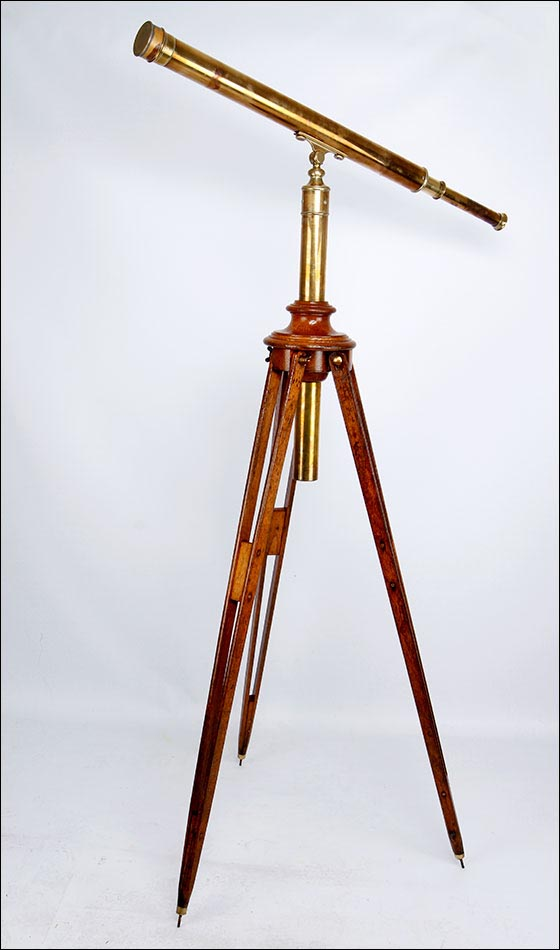
\includegraphics[width=0.6\textwidth]{images/telescopio_antiguo.jpg}
	\caption{Telescopio antiguo, aproximadamente de principios de los 1800.}
	\label{fig:telescopio_antiguo}
\end{figure}

Históricamente, la patente original de un telescopio refractor fue registrada por Hans Lipperhey, un fabricante de lentes de Middelburg (Países Bajos), aunque existen discrepancias sobre si fue realmente su inventor, puesto que existen registros antiguos de marinos que ocupaban lentes para observar las costas en el horizonte. Con la diseminación por Europa de la noticia sobre este instrumento óptico, Galileo Galilei tuvo conocimiento de él, lo cual le llevó a construir una versión propia y la utilizó para observar el cielo nocturno. Así logró ver objetos invisibles al ojo humano, como las lunas de Júpiter y estrellas ubicadas en regiones aparentemente “vacías” del cielo.

Ese momento marcó un punto de inflexión en la historia del conocimiento: por primera vez, se accedía a una visión detallada del universo que desafiaba las ideas establecidas sobre nuestra posición en el cosmos.

\begin{figure}[H]
	\centering
	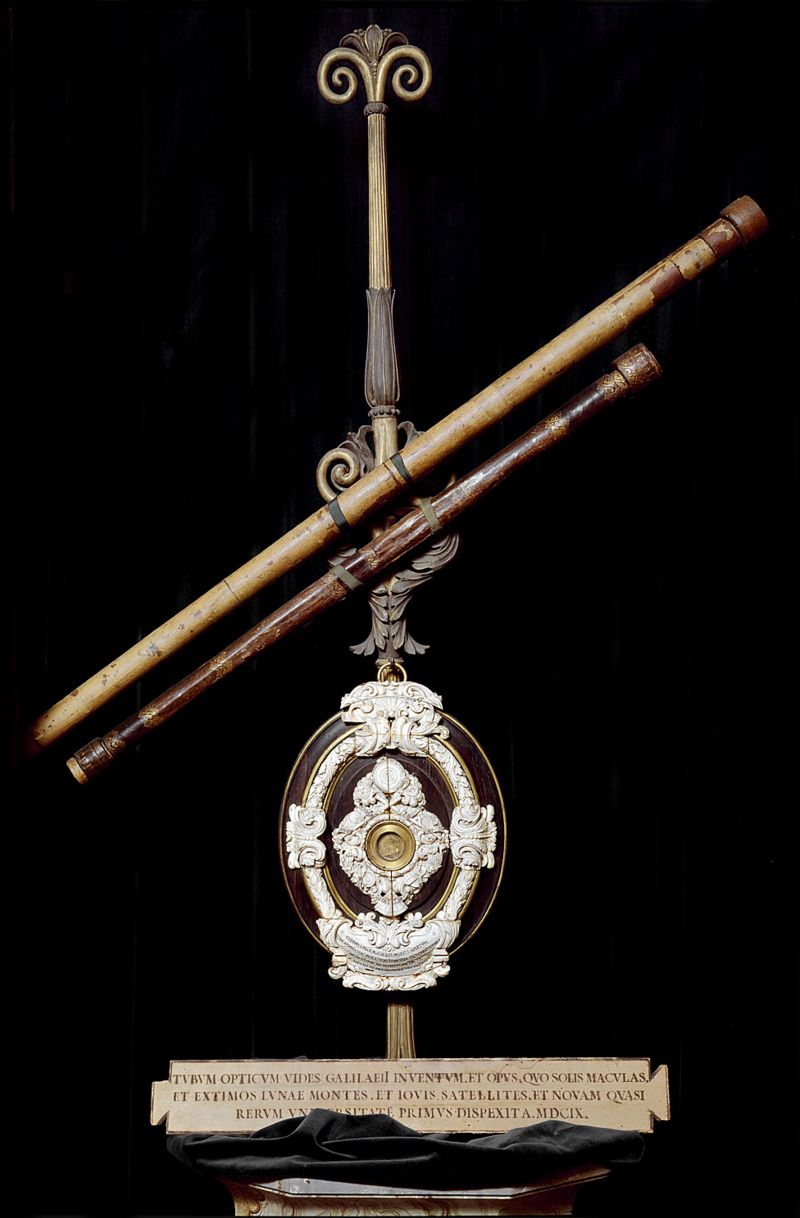
\includegraphics[width=0.6\textwidth]{images/telescopio_galileo.jpg}
	\caption{Versión modificada de telescopios tradicionales hecha por Galileo para poder captar mejor objetos lejanos.}
	\label{fig:telescopio_patente_galileo}
\end{figure}
% SUGERENCIA: insertar un video corto o animación de las lunas de Júpiter orbitando.
% También podría incluirse una ilustración de Galileo observando con su telescopio.

El término telescopio abarca una amplia variedad de dispositivos: radiotelescopios, telescopios infrarrojos y ultravioletas, así como telescopios ópticos. En este documento nos enfocaremos en estos últimos, que son los más comunes y accesibles, ideales para introducirse al mundo de la observación astronómica.

Esta guía forma parte del minicurso organizado por la Comisión de Creación de Telescopios del Capítulo de Óptica de Yachay Tech, realizado en abril de 2024.

\subsection*{Breve historia del telescopio}

El registro más antiguo sobre la existencia de uso de un telescopio refractor corresponde a una patente solicitada por Hans Lippershey, en los Países Bajos en el siglo XVII, pese a que no se la otorgó el diseño del instrumento se popularizó alrededor de Europa, y fue en 1609 cuando Galileo Galilei lo empleó con fines astronómicos para observar el cielo, marcando un hito en la historia de la ciencia. Esto debido a que sus resultados respaldaban la teoría heliocentrista y se iba en contra lo aceptado, la teoría geocéntrica, donde se asume que la tierra es el centro del universo, donde los planetas, la luna y las estrellas giran alrededor nuestro. Galileo no sólo tomaba nota de sus observaciones, sino que también creaba ilustraciones de sus hipótesis (fig \ref{fig:ilustracion_luna_galileo_1610}). Finalmente, a esta revolución de la ciencia se incluye Johannes Kepler, quien mejora el invento de Galileo otorgando un mayor campo de visión siendo el precursor de los telescopios astronómicos modernos, aunque invierte la imagen. 

\begin{figure}[H]
	\centering
	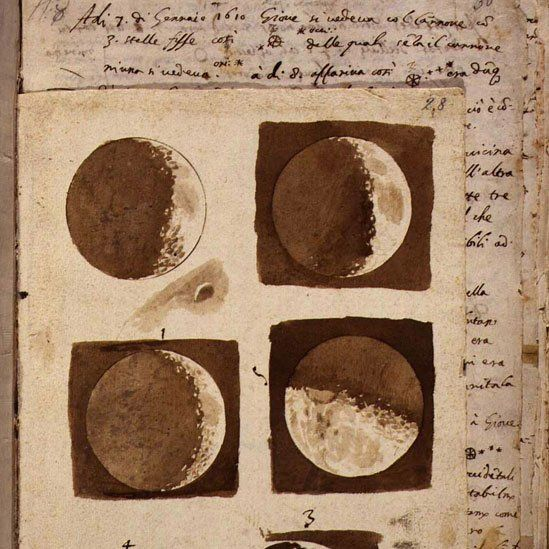
\includegraphics[width=0.6\textwidth]{images/ilustracion_galileo.jpg}
	\caption{Ilustración de la Luna hecha por Galileo Galilei en 1610. Presentada en su obra Siderus Nuncius.}
	\label{fig:ilustracion_luna_galileo_1610}
\end{figure}

Con el tiempo, se empezó a investigar el uso de espejos para captar luz, en lugar de lentes. Esto permitía evitar problemas comunes en los telescopios que usan lentes. En 1668, Isaac Newton construyó el primer telescopio reflector funcional, conocido hoy como Telescopio Reflector Newtoniano (\ref{fig:telescopio_reflector_newotoniano}). Este invento ocupa un espejo cóncavo en lugar de lentes para evitar aberraciones cromáticas. 

Las principales diferencias entre estos dos tipos de telescopios vienen dados en la siguiente tabla:
 
\begin{table}[h!]
\centering
\caption{Tabla comparativa de telescopios refractarios vs reflectores}
\begin{tabular}{ |p{3cm}||p{3cm}|p{3cm}|p{3cm}|  }
	\hline
	\multicolumn{4}{|c|}{Telescopes comparison} \\
	\hline
	 & Refractor & Reflector & Mezcla \\
	\hline
	Materiales & AF    &AFG&   004\\
	Ventajas&   AX  & ALA   &248\\
	Fabricación &AL & ALB&  008\\
	Limitantes &DZ & DZA&  012\\
	\hline
\end{tabular}
\end{table}
% SUGERENCIA: incluir una tabla comparativa simple: refractor vs reflector (material, ventajas, época).
% O una ilustración estilo línea de tiempo con telescopios clave.

Durante más de un siglo, los telescopios refractores evolucionaron lentamente, hasta que en 1730 se desarrollaron lentes acromáticas, lo que mejoró significativamente la calidad de imagen. Por otro lado, los primeros telescopios reflectores enfrentaban un problema relacionado con la pérdida de brillo en los espejos metálicos (fig \ref{fig:espejo_metalico_especulum}). Este problema se fue solucionado progresivamente en la década de 1850 con la introducción de espejos de vidrio recubiertos, y más adelante, en 1932, con la implementación de espejos aluminizados.

\begin{figure}[H]
	\centering
	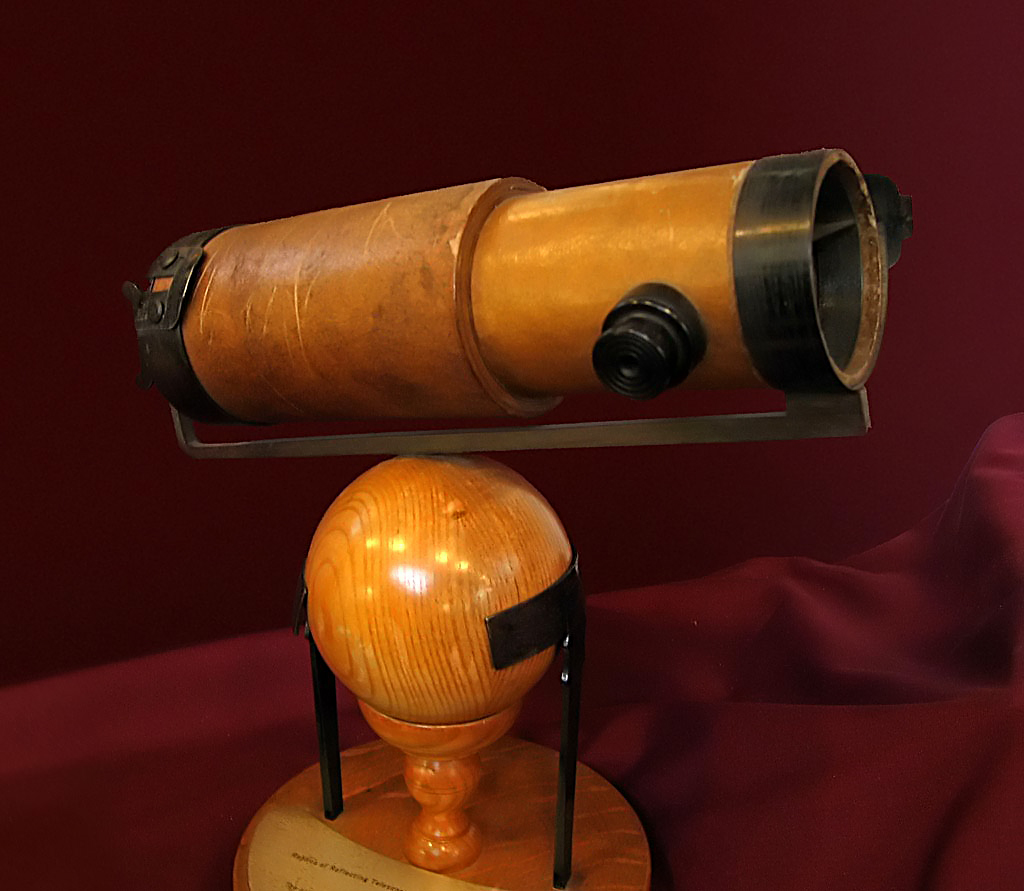
\includegraphics[width=0.6\textwidth]{newton_reflector_telescopio.jpg}
	\caption{Réplica del primer telescopio reflector registrado por Isaac Newton ante la Royal Society en 1672.}
	\label{fig:telescopio_reflector_newotoniano}
	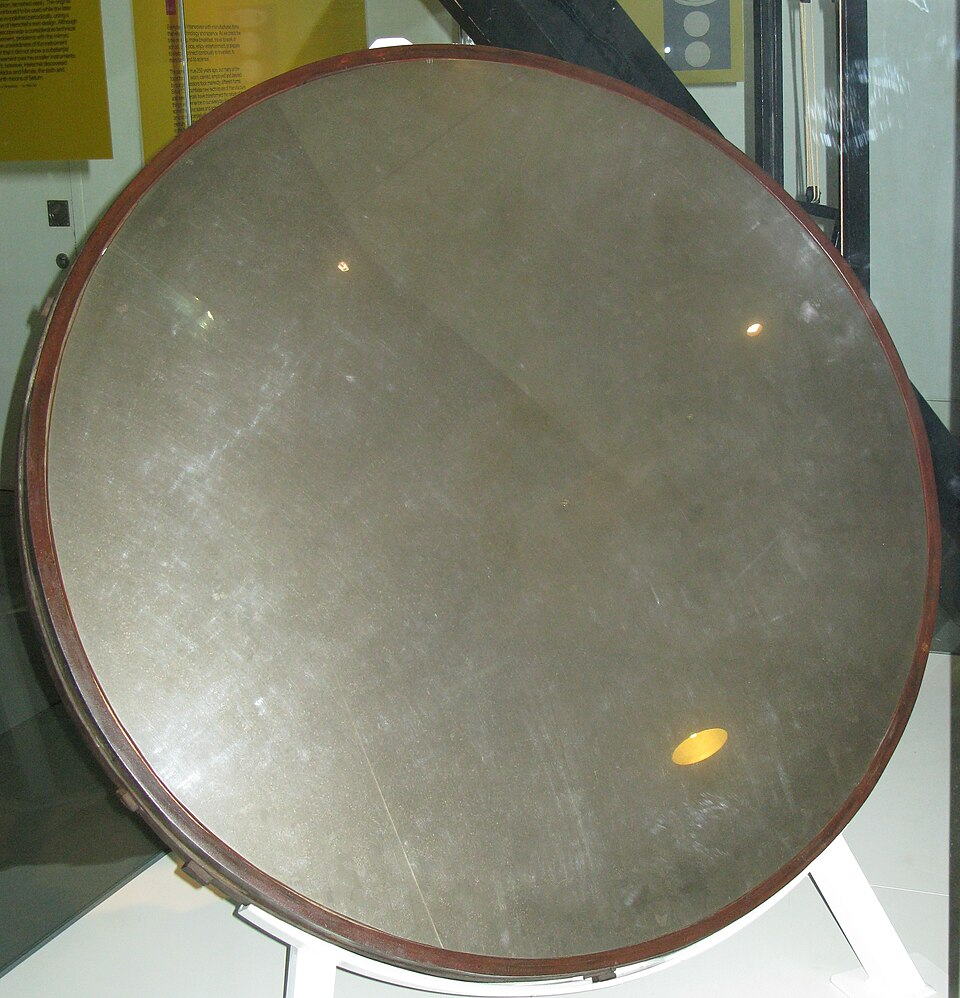
\includegraphics[width=0.6\textwidth]{speculum_mirror_metal.jpg}
	\caption{Espejo metálico de 1.2m de diámetro para un telescopio de 40pies.}
	\label{fig:espejo_metalico_especulum}
\end{figure}

En aquella época, los telescopios refractores más grandes alcanzaban aperturas de aproximadamente $1\,\mathrm{m} \approx 39\,\mathrm{in}$, mientras que los reflectores superaban los $10\,\mathrm{m} \approx 33\,\mathrm{ft}$. Actualmente, se están construyendo telescopios aún más grandes, con aperturas entre $30$ y $40\,\mathrm{m}$, telescopios que se ubican en órbita para evitar interferencias con la atmósfera. Sin embargo, la utilización de telescopios ópticos terrestres continúa siendo de gran interés científico debido a las nuevas tecnologías las cuales ofrecen soluciones adaptativas, de bajo costo y gran impacto en investigación. Además de los nuevos algoritmos de procesamiento de imágenes y de corrección de aberraciones ofrecen un gran marco teórico para el desarrollo de instrumentos ópticos (fig \ref{fig:gran_telescopio_canarias} \ref{fig:gmt_chile}). 

\begin{figure}[H]
	\centering
	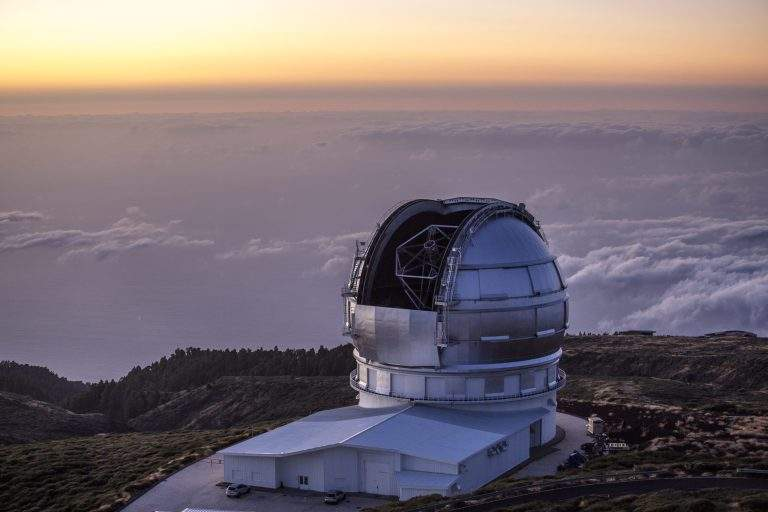
\includegraphics[width=0.6\textwidth]{gran_telescopio_canarias.jpg}
	\caption{Gran telescopio de Canarias (GTC). Telescopio reflector con 10.4m de diámetro de espejo principal, compuesto por 36 segmentos hexagonales.}
	\label{fig:gran_telescopio_canarias}
	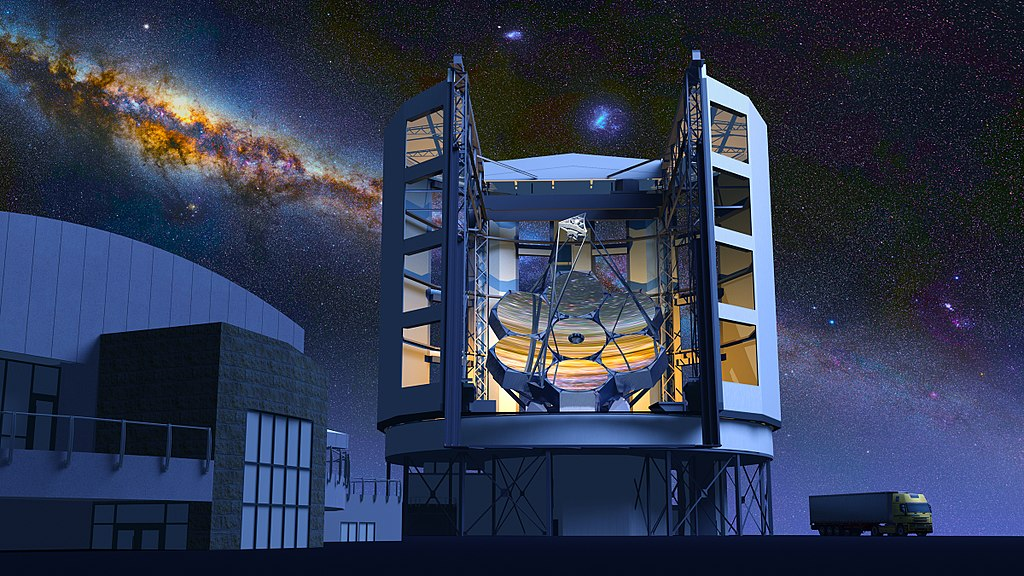
\includegraphics[width=0.6\textwidth]{giant_magallan_telescope.jpg}
	\caption{Giant Magellan Telescope (GMT) es uno de los tres proyectos de telescopios más grandes actualmente en construcción, en el desierto de Atacama - Chile.}
	\label{fig:gmt_chile}
\end{figure}


 
% SUGERENCIA: 
% insertar una animación con transición de escalas.


\section{Principios Ópticos Fundamentales}
\subsection*{La luz y su velocidad}

La luz, tal como la percibimos, corresponde a una fracción del espectro electromagnético la cual puede ser detectada por nuestro sistema visual. Su definición, en términos prácticos, está íntimamente relacionada con la respuesta fisiológica y psicológica del sistema ojo-cerebro frente a estímulos dentro del rango de la luz visible, que abarca frecuencias entre $400$ y $700 nm$.

Por ejemplo, una mezcla de luz roja y verde es interpretada por nuestro sistema visual como luz amarilla, aunque no exista radiación electromagnética en la longitud de onda correspondiente al amarillo. Este fenómeno se conoce como \textit{mezcla aditiva de colores} y es una propiedad emergente de cómo procesamos la luz, más que de la luz en sí misma.

\vspace{0.3cm}
% FIGURA sugerida: diagrama con el espectro visible y un círculo de mezcla RGB

%\subsection{Breve historia de la medición de la velocidad de la luz}

Desde hace siglos, el ser humano ha intentado determinar si la luz tiene velocidad finita o es instantánea. Con el desarrollo de los telescopios, comenzaron a surgir los primeros experimentos.

%\subsubsection{Intento de Galileo}

Galileo Galilei, en el siglo XVII, intentó medir la velocidad de la luz con la ayuda de un asistente. Cada uno portaba una linterna, y se situaban a unos 3 kilómetros de distancia. Galileo destapaba su linterna, y cuando su asistente veía la luz, destapaba la suya en respuesta. Galileo cronometraba el tiempo entre su acción inicial y la recepción de la segunda luz.

Aunque ingenioso, el experimento no tuvo éxito. Hoy sabemos que la luz recorre 3 kilómetros en aproximadamente $10^{-5}$ segundos, un tiempo imposible de medir con instrumentos de la época, además no se consideraba el factor de error humano, donde ni con los reflejos entrenados puede responder a estímulos de tal velocidad.


\vspace{0.3cm}
% ILUSTRACIÓN sugerida: recreación simple del experimento con linternas

%\subsubsection{Ole Rømer y las lunas de Júpiter}

En 1675, el astrónomo danés Ole Rømer estudió durante varios años los eclipses de la luna Io, una de los satélites naturales de Júpiter. Rømer, observó que la duración entre eclipses variaba dependiendo de la posición relativa entre la Tierra y Júpiter. Cuando la Tierra se alejaba de Júpiter, los eclipses parecían retrasarse.

Rømer concluyó correctamente que la luz tardaba un tiempo finito en viajar, y que esta diferencia se debía al cambio en la distancia. Su trabajo fue el primer indicio experimental de que la luz no tenía velocidad infinita.

\vspace{0.3cm}
% ILUSTRACIÓN sugerida: esquema Tierra-Júpiter con Io mostrando trayectos de luz más largos/cortos

% \subsection{James Bradley}

Por otro lado, James Bradley, un físico de Inglaterra con la ayuda de telescopios descubre, por serendipia, un cambio simétrico (paralaje), es decir, observó el desplazamiento cíclico de toda la esfera celeste a lo largo del año, con un pico máximo de cambio, lo que ocurría con la tierra con una velocidad orbital dada, lo que se explicaba con el movimiento de la tierra alrededor del sol, respaldando la teoría heliocentrista, y por una velocidad finita de la luz. Estimó $\sim 301,000 km/s$.



%\subsubsection{Método de Fizeau (1849)}

% En 1849, el físico francés Hippolyte Fizeau diseñó un ingenioso experimento para medir la velocidad de la luz en laboratorio. Utilizó una rueda dentada giratoria y un haz de luz que atravesaba uno de los espacios entre los dientes hacia un espejo situado a unos 8 km de distancia. El haz se reflejaba y regresaba a través de la misma rueda.

% Cuando la rueda giraba a una velocidad específica, el haz reflejado era bloqueado por el siguiente diente. Midiendo esa velocidad de rotación y la distancia al espejo, Fizeau logró estimar el tiempo de viaje de la luz y, con ello, su velocidad.

% Este fue el primer experimento exitoso para medir la velocidad de la luz sin necesidad de observaciones astronómicas.

\vspace{0.3cm}
% FIGURA sugerida: diagrama de la rueda dentada, fuente de luz, espejo a distancia

%\subsubsection{Método de Michelson (1879)}

% Albert A. Michelson, en 1879, perfeccionó el método de Fizeau. En lugar de una rueda dentada, utilizó un espejo giratorio de alta precisión. El haz de luz se reflejaba hacia un espejo fijo a varios kilómetros, y luego regresaba.

% Durante ese tiempo, el espejo giratorio cambiaba de orientación, lo que hacía que el haz de retorno se desviara. Midiendo con precisión ese ángulo de desviación, Michelson pudo calcular con mayor exactitud el tiempo de viaje de la luz y, por lo tanto, su velocidad.

% Este método se convirtió en uno de los más confiables del siglo XIX, y Michelson fue reconocido con el Premio Nobel en 1907, siendo el primer estadounidense en recibirlo por un trabajo de física.

\vspace{0.3cm}
% FIGURA sugerida: diagrama del espejo giratorio y trayectoria desviada del haz

%\subsection{Relación con las constantes electromagnéticas}

Hoy en día, uno de los métodos más exactos para conocer la velocidad de la luz es a través de las constantes del electromagnetismo. La relación fundamental es:

\[
c = \frac{1}{\sqrt{\epsilon_0 \mu_0}}
\]

Donde:
\begin{itemize}
	\item $\epsilon_0$ es la permitividad eléctrica del vacío ($8.854 \times 10^{-12}\, \text{F/m}$),
	\item $\mu_0$ es la permeabilidad magnética del vacío ($4\pi \times 10^{-7}\, \text{N/A}^2$).
\end{itemize}

Esta ecuación, derivada de las ecuaciones de Maxwell, describe cómo los campos eléctricos y magnéticos se propagan en el vacío. A partir de estas constantes, se puede demostrar que la velocidad de propagación de cualquier onda electromagnética en el vacío es constante y finita, por lo tanto siendo la luz una perturbación del campo electromagnético, la velocidad de la luz en el vacío es constante y finita: 
(añadir anexos con los calculos para esto)

\begin{mybox}[blue]{Velocidad de la luz en el vacío}[colbacktitle=blue!30!white, coltitle=black]
	$c = 299\,792\,458 \, \text{m/s} \approx 3\cdot10^8 \text{m/s}$ 
\end{mybox}



\vspace{0.3cm}
% FIGURA sugerida: resumen visual con ecuación, valor de c, y conexión con unidades SI

%\begin{mybox}[green]{Espacio Vectorial}[colbacktitle=blue!30!white, coltitle=black]
%	Un conjunto con dos operaciones (suma y producto por escalar) que satisfacen 8 axiomas.
%\end{mybox}
%
%\begin{mybox}[gray]{Espacio Vectorial}[colbacktitle=blue!30!white, coltitle=black]
%	Un conjunto con dos operaciones (suma y producto por escalar) que satisfacen 8 axiomas.
%\end{mybox}

\section*{Propagación de la luz}

La propagación de la luz, al tratarse de una oscilación del campo electromagnético, está regida por la ecuación de onda. No obstante, mucho antes de que Maxwell desarrollara la teoría del electromagnetismo, la propagación de la luz ya había sido descrita empíricamente mediante dos principios fundamentales: el Principio de Huygens y el Principio de Fermat.

El principio de Huygens, propuesto por el físico holandés Christiaan Huygens en el siglo XVII, describe el comportamiento de los frentes de onda de forma geométrica:

\begin{mybox}[green]{Principio de Huygens}[colbacktitle=blue!30!white, coltitle=black]
	Cada punto de un frente de onda primario actúa como foco, o fuente, de ondas esféricas secundarias que se propagan con la misma velocidad y frecuencia que la onda original. El nuevo frente de onda, al cabo de un intervalo de tiempo, es la envolvente de estas ondas secundarias.
\end{mybox}

Por otro lado, el principio de Fermat, basado en una idea geométrica y variacional, establece:

\begin{mybox}[green]{Principio de Fermat}[colbacktitle=blue!30!white, coltitle=black]
	La trayectoria que sigue la luz al pasar de un punto \textbf{A} a un punto \textbf{B} es aquella en la que el tiempo de recorrido es mínimo. Es decir, la luz tiende a seguir el camino óptico más rápido.
\end{mybox}

\vspace{0.3cm}
% FIGURA SUGERIDA: Comparación visual de Huygens y Fermat con una superficie separadora aire-vidrio

Estos principios no solo son compatibles, sino que se complementan. El primero ofrece una visión geométrica local, útil para explicar fenómenos como la difracción, mientras que el segundo permite deducir leyes globales como la de la refracción.

\section{Reflexión y Refracción}

La velocidad de la luz en medios transparentes como el aire, el agua o el vidrio es menor que su velocidad en el vacío. Esta diferencia da lugar a un parámetro óptico llamado \textbf{índice de refracción}, este está definido como:

\begin{mybox}[blue]{Índice de refracción}[colbacktitle=blue!30!white, coltitle=black]
	$n = \frac{c}{v}$
\end{mybox}

donde:
\begin{itemize}
	\item $c$ es la velocidad de la luz en el vacío,
	\item $v$ es la velocidad de la luz en el medio considerado.
\end{itemize}

Cuando un rayo de luz incide sobre la interfaz entre dos medios con diferente índice de refracción (por ejemplo, aire y vidrio), una parte de la energía se refleja y otra parte penetra en el segundo medio, cambiando de dirección: este fenómeno se conoce como \textbf{refracción}.

% FIGURA: ya está incluida: refraction_reflection.png

\begin{figure}[H]		
	\centering
	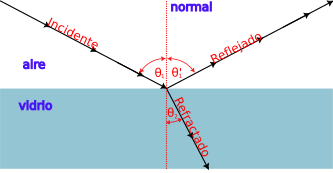
\includegraphics[width=0.6\textwidth]{images/refraction_reflection.png}
	\caption{El ángulo de reflexión es igual al ángulo de incidencia. El ángulo de refracción $\theta_2$ depende de la relación entre las velocidades de propagación en ambos medios.}
	\label{fig:refraccón_reflexión_planos}
\end{figure} 

En la figura \ref{fig:refraccón_reflexión_planos} se observa un rayo de luz incidente sobre la superficie de un vidrio. El ángulo $\theta_1$ entre el rayo incidente y la normal se denomina \textbf{ángulo de incidencia}, y el plano definido por ambos se llama \textbf{plano de incidencia}.

El rayo reflejado se encuentra en el mismo plano y forma un ángulo igual con la normal, lo cual se expresa con la \textbf{ley de la reflexión}:

\begin{mybox}[blue]{Ley de la reflexión}[colbacktitle=blue!30!white, coltitle=black]
	$\theta'_1 = \theta_1$
\end{mybox}

Por otro lado, el rayo que entra al segundo medio (el rayo \textbf{refractado}) cambia de dirección debido al cambio de velocidad de propagación. La relación entre los ángulos y las velocidades en cada medio se expresa como:

\begin{equation}
	\frac{1}{v_1} \sin(\theta_1) = \frac{1}{v_2} \sin(\theta_2)
	\label{eq:refraccion_dos_medios}
\end{equation}

Si sustituimos las velocidades por sus respectivas expresiones en términos del índice de refracción ($v = c/n$), obtenemos la conocida \textbf{ley de Snell}:

\begin{mybox}[blue]{Ley de Snell de la refracción}[colbacktitle=blue!30!white, coltitle=black]
	$n_1 \sin(\theta_1) = n_2 \sin(\theta_2)$
\end{mybox} 

\vspace{0.3cm}
% FIGURA sugerida extra (opcional): simulación de cómo cambia el ángulo de refracción con diferentes índices

\subsection{Mecanismos físicos de la reflexión y la refracción}

A nivel microscópico, la reflexión y la refracción pueden entenderse como fenómenos de interacción entre la luz y los átomos del medio. Cuando un rayo de luz incide sobre una superficie, sus campos eléctricos hacen oscilar las cargas (principalmente electrones) en los átomos del material. Estas oscilaciones inducidas producen una nueva radiación: la luz es absorbida y reemitida por los átomos.

En el fenómeno de la reflexión, parte de las ondas reemitidas se propagan en dirección opuesta al haz de luz incidente. Debido a interferencias constructivas (coherencia de la onda incidente) estas ondas se reflejan constructivamente en una dirección bien definida, formando el rayo reflejado. 

En el caso de la refracción, la luz reemitida hacia adelante también sufre interferencia constructiva, pero en una dirección distinta a la original. El resultado neto es un cambio en la dirección de propagación, determinado por la diferencia de velocidades de fase en cada medio.



% NOTA: esta explicación es un paso hacia modelos electromagnéticos, pero aún accesible a estudiantes de primeros semestres

\subsection*{Reflexión Especular y Difusa}

La reflexión especular ocurre en superficies suaves y lisas. Podemos observar en la imagen \ref{fig:ref_especular_difusa} donde los rayos de luz del objeto $P$ al reflejar en el espejo forman una imagen como si procediecen del punto $P'$, este se denomina \textbf{imagen virtual del punto $P$}.
Por otro lado, la reflexión difusa ocurre cuando la superficie donde se refleja la imagen es rugisa, es decir, los rayos procedentes de un puesto se reflejan en todas direcciones y no divergen de ningún punto. 

\begin{figure}[H]
	\centering
	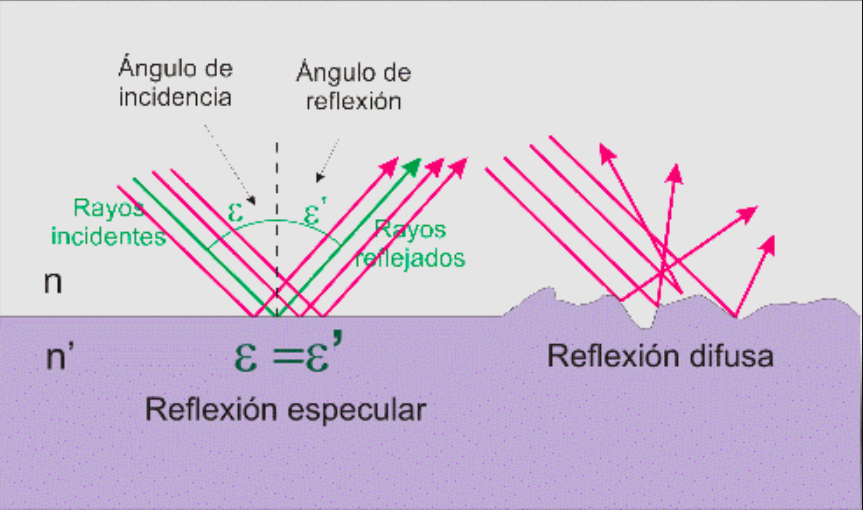
\includegraphics[width=0.6\textheight]{ref_especular_difusa.png}
	\caption{Reflexion especular y difusa.}
	\label{fig:ref_especular_difusa}
\end{figure}

% Intensidad de relativa de la luz reflejada y transmitida
% Reflexión interna total
%% Fibra óptica
% Espejismo

\subsection*{Dispersión}

El índice de refracción de un material depende ligeramente de la longitud de onda con la que incide un haz de luz. Para la mayoría de materiales, $n$ disminuye cuando crece la longitud de onda. La dependencia entre el índice de refracción con la longitud de onda (y por tanto con la frecuencia) se denomina \textbf{dispersión}.

\begin{figure}[H]
	\centering
	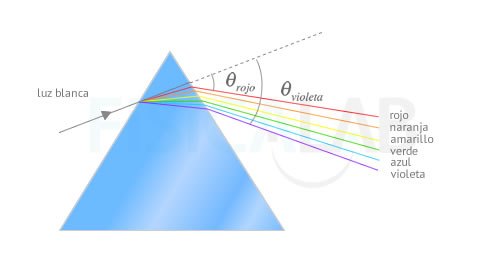
\includegraphics[width=0.6\textwidth]{images/descomposicion_luz.jpg}
	\caption{Imagen de la descomposición de la luz blanca cuando atraviesa un prisma.}
	\ref{fig:dispersion_prisma_luz}
\end{figure}

% Arcoiris.

% Polarización
%% Polarización por absorción
%% Polarización por reflexión
%% Polarización por dispersión(o scattering)
%% Polarización por birrefringencia


% Dualidad Onda- Partícula
% Espectros de Luz
% Fuentes luminosas, líneas espectrales

\subsection{Reflexión y espejos}

\subsubsection*{Espejos Planos}
Los espejos planos, los más conocidos. Podemos observar la figura \ref{fig:espejos_planos}, en ella se ilustran dos rayos que se emiten de los extremos de la botella (en realidad van en todas las direcciones), estos son los que encierra el haz de rayos de luz que entra al ojo. Cada conjunto de rayos divergentes que se reflejan en el espejo y entran en el ojo parecen provenir de un mismo punto (llamado punto de imagen) detras del espejo, tal y como muestran las líneas punteadas. Siempre que un objeto esté dentro del plano de un espejo existe una posición en la cual puede situarase el ojo para poder ver la imagen. 

\begin{figure}[H]
	\centering
	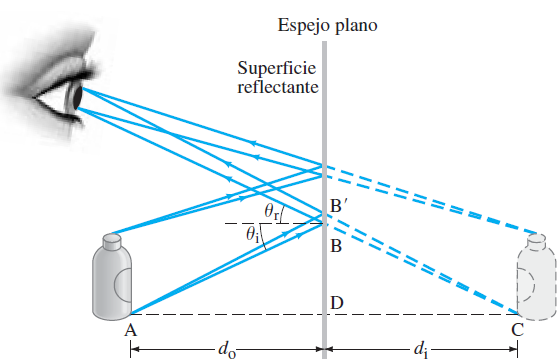
\includegraphics[width=0.6\textwidth]{images/espejo_plano.png}
	\caption{Espejo plano reflejando una botella. Se marcan los puntos que son los que entrarán al ojo.}
	\label{fig:esplejos_planos}
\end{figure}

En los espejos también podemos observar el resultado de inversión en profundidad, es decir, si ponemos la mano derecha en el espejo vemos convertida en la mano izquierda, también podemos observarlo como un cambio de coordenadas, donde el espejo transforma un sistema de coordenadas según la regla de la mano derecha, donde $\hat{i} \times \hat{j} = \hat{k}$ se convierte en $\hat{i} \times \hat{j} = -\hat{k}$. 

\begin{figure}[H]
	\centering
	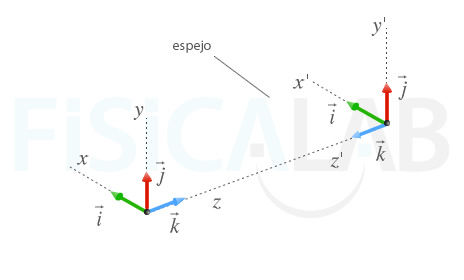
\includegraphics[width=0.6\textwidth]{images/inversion_profundidad.jpg}
	\caption{.}
	\label{fig:inversion_profundidad}
\end{figure}

\subsubsection*{Espejos Esféricos}

Podemos observar la figura \ref{fig:espejo_esferico}, que muestra un haz de rayos que provienen del punto $P$ situado en el eje de un espejo esférico cóncavo y  que después de reflejarse en él convergen en el punto $P'$, también denominado \textbf{imagen real}. Se le denomina imagen real porque la luz realmente emana del punto imagen, esta puede ser vista por cualquier observador al lado izquierdo del espejo. (Regresar a la explicación de imagenes virtuales en espejos planos). 

\begin{figure}[H]
	\centering
	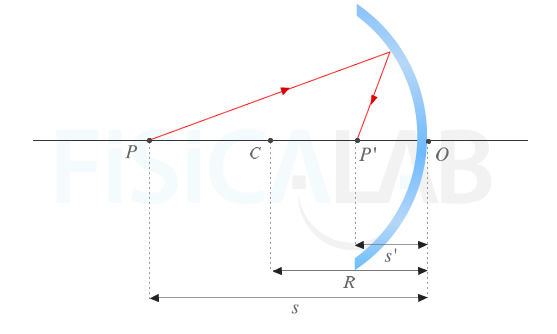
\includegraphics[width=0.6\textwidth]{images/espejo_esferico_AV.jpg}
	\caption{Los rayos procedientes del punto $P$, en el eje $PO$ de un espejo esférico concavo forman una imagen en $P'$. Los rayos más significativos son los que inciden más cercanos al eje $PO$.}
	\label{fig:espejo_esferico}
\end{figure}

En los espejos cóncavos también se pueden generar aberraciones denominadas \textbf{aberraciones esféricas}. Los rayos que rebotan más lejanos al eje $PO$ son los causantes de estas aberraciones, esto es debido a que estos rayos no consiguen pasar exactamente por el punto de la imagen.

Para cálculos relacionados a espejos esféricos queremos buscar una ecuación que relacione el punto $P$ con el punto $P'$. 

\begin{figure}[H]
	\centering
	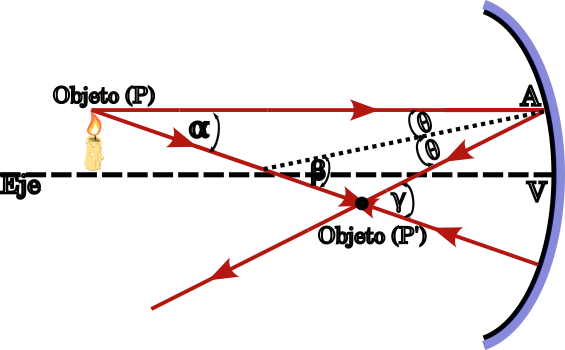
\includegraphics[width=0.6\textwidth]{images/geometria_espejos.png}
	\caption{Geometría para espejos}
	\label{fig:geometria_espejos_imagen}
\end{figure}

Siguiendo identidades trigonométricas, se llega a la conclusión de que 
\begin{equation}
	\alpha + \gamma = 2\beta
\end{equation}


\subsection{Refracción y Lentes}
Para crear lentes se pulen cilindros de vidrio para formar superficies esféricas convexas. Suponiendo que todos los rayos son paraxiales, mediante la aproximación de ángulos pequeños tenemos $\alpha \approx l/s$, $\beta = \approx l/r$, $\gamma = l/s'$. 

\begin{equation}
	\frac{1}{s} + \frac{1}{s'} = \frac{2}{r}
\end{equation}



\subsection{Combinación Lentes-Espejos}


\section{Tipos de Telescopios}
% Tipos y características
\subsection{Telescopios Refractores}

\subsection{Telescopios Reflectores}

\subsection{Telescopios Catadióptricos}

\section{Parámetros Clave de un Telescopio}

\subsection{Apertura}
\subsection{Distancia Focal}
\subsection{Relación Focal}
\subsection{Aumento y Resolución}

\section{Monturas de Telescopios}
\subsection{Montura Altazimutal}
\subsection{Montura Ecuatorial}
\subsection{Montura Dobson}

\section{Grandes Telescopios y Futuro en Astronomía}

El estado del arte de los telescopios en tierra es muy prometedor. Existen proyectos próximos a entrar en funcionamiento, tales como el Observatorio Vera C. Rubin, el cual hará uso del sensor más grande construido desde un principio con enfoque en astronomía. Este sensor cuenta con 3200 megapixeles, que permitirá que cada imagen tome una fotografía con una extensión similar a 40 lunas llenas (referencia- https://elpais.com/chile/2024-12-27/el-telescopio-con-la-mayor-camara-digital-del-mundo-construida-para-la-astronomia-se-asoma-en-una-montana-chilena.html ) las operaciones están previstas empezar en 2028. El proyecto lleva a cabo el consorcio de universidades estadounidenses AURA yy afiliados internacionales. 
% Mencionar algunos telescopios terrestres importantes como el Gran Telescopio de Canarias (GRANTECAN), el Very Large Telescope (VLT), y observatorios como el de Mauna Kea.
% Resaltar la importancia de los telescopios espaciales como el Hubble y el James Webb. Su ubicación fuera de la atmósfera proporciona imágenes más nítidas.
% Introducción a futuros telescopios como el Extremely Large Telescope (ELT) y el Wide Field Infrared Survey Telescope (WFIRST)

\section{Consideraciones para la Elección de un Telescopio}

\section{Preguntas y Discusión}

	
	\chapter{Solidworks - Modelado por CAD de un Telescopio}
	\label{solidworks_focused_telescopes}
	\section{Introducción al Diseño CAD}

\subsection{Mentalidad de diseño CAD}
%\begin{itemize}
%	\item Pensar en términos de geometrías simples.
%	\item Enfoque práctico para abordar problemas de diseño.
%\end{itemize}

\subsection{Introducción a SolidWorks y software CAD similares}
%\begin{itemize}
%	\item SolidWorks, Fusion 360, Inventor, FreeCAD.
%	\item Importancia de conceptos comunes (paramétricos).
%\end{itemize}

\section{Principios Geométricos Básicos}

\subsection{Elementos básicos}
%\begin{itemize}
%	\item Puntos, líneas y planos.
%	\item Sistema de coordenadas cartesianas (X, Y, Z).
%\end{itemize}

\subsection{Ángulos y trigonometría básica}
%\begin{itemize}
%	\item Definiciones básicas de ángulos y triángulos.
%	\item Aplicación sencilla en CAD.
%\end{itemize}

\subsection{Restricciones geométricas y transformaciones}
%\begin{itemize}
%	\item Relaciones: paralelo, perpendicular, coincidente, etc.
%	\item Movimientos, rotaciones y escalado.
%\end{itemize}

\section{Interfaz Esencial de SolidWorks}

\subsection{Herramientas básicas de interfaz}
%\begin{itemize}
%	\item Barra de menú superior.
%	\item Command Manager.
%	\item Feature Manager Design Tree.
%	\item Área gráfica (Graphics Area).
%\end{itemize}

\subsection{Navegación básica del modelo}
%\begin{itemize}
%	\item Rotación y zoom con el mouse.
%	\item Vistas estándar (superior, frontal, lateral).
%\end{itemize}

\subsection{Árbol de diseño (Feature Manager)}
%\begin{itemize}
%	\item Historial de diseño y jerarquía de operaciones.
%	\item Operaciones padres e hijos.
%\end{itemize}

\section{Flujo de Trabajo CAD para Telescopios}

\subsection{Definición del problema de diseño}
%\begin{itemize}
%	\item Identificación de piezas clave (tubos, espejos, monturas).
%\end{itemize}

\subsection{Descomposición geométrica del telescopio}
%\begin{itemize}
%	\item Formas básicas: cilindros, discos, placas.
%\end{itemize}

\subsection{Construcción gradual del modelo}
%\begin{itemize}
%	\item Secuencia: boceto $\rightarrow$ operación 3D $\rightarrow$ ensamblaje.
%\end{itemize}

\section{Bocetos 2D (Sketches)}

\subsection{Conceptos iniciales}
%\begin{itemize}
%	\item Uso de planos predeterminados (Front, Top, Right).
%	\item Creación de nuevos planos.
%\end{itemize}

\subsection{Herramientas básicas de boceto}
%\begin{itemize}
%	\item Línea, círculo, rectángulo, polígono, spline.
%	\item Líneas constructivas.
%\end{itemize}

\subsection{Relaciones geométricas esenciales}
%\begin{itemize}
%	\item Coincidente, tangente, paralelo, igual, etc.
%\end{itemize}

\subsection{Cotas inteligentes}
%\begin{itemize}
%	\item Definir dimensiones y posiciones.
%	\item Importancia de bocetos completamente definidos.
%\end{itemize}

%\subsection{Práctica rápida}
%\begin{itemize}
%	\item Sección transversal de un tubo óptico.
%\end{itemize}

\section{Operaciones 3D Fundamentales para Telescopios}

\subsection{Extrusiones básicas}
%\begin{itemize}
%	\item Tubos, adaptadores y bases planas.
%\end{itemize}

\subsection{Revoluciones básicas}
%\begin{itemize}
%	\item Modelado de piezas cilíndricas y espejos parabólicos.
%\end{itemize}

\subsection{Operaciones de corte}
%\begin{itemize}
%	\item Cortes por extrusión y revolución.
%\end{itemize}

\subsection{Redondeos y chaflanes}
%\begin{itemize}
%	\item Suavizar aristas para impresión o montaje.
%\end{itemize}

\subsection{Patrones circulares y lineales}
%\begin{itemize}
%	\item Distribución simétrica de agujeros o soportes.
%\end{itemize}

%\subsection{Ejercicios prácticos}
%\begin{itemize}
%	\item Diseño de tubo para ocular.
%	\item Espejo primario básico por revolución.
%\end{itemize}

\section{Ensamblajes Básicos de Telescopios}

\subsection{Inserción y posicionamiento de piezas}
%\begin{itemize}
%	\item Insertar componentes.
%	\item Relaciones: concéntrica, coincidente, distancia.
%\end{itemize}

\subsection{Ejemplo de ensamblaje}
%\begin{itemize}
%	\item Ensamble simple: tubo + espejo + soporte.
%\end{itemize}

%\section{Dibujos Técnicos para Fabricación}


%\subsection{Creación de vistas técnicas}
%\begin{itemize}
%	\item Vistas frontal, lateral, superior, isométrica.
%\end{itemize}

\subsection{Acotado de piezas}
%\begin{itemize}
%	\item Uso de cotas inteligentes en vistas.
%\end{itemize}

\subsection{Exportación}
%\begin{itemize}
%	\item Exportar a PDF o plano físico.
%	\item Exportar bonito, para no perder los paths. 
%\end{itemize}

\section{Consejos para Fabricación con Impresión 3D}

\subsection{Preparación del modelo}
%\begin{itemize}
%	\item Inclinación, soporte, grosor mínimo.
%\end{itemize}

\subsection{Alternativas prácticas}
%\begin{itemize}
%	\item Uso de PVC, madera, corte láser.
%\end{itemize}

\subsection{Exportación a STL}
%\begin{itemize}
%	\item Preparar archivo para impresión 3D.
%\end{itemize}

\section{Preguntas y Revisión Final}
%
%\begin{itemize}
%	\item Espacio abierto para dudas.
%	\item Revisión rápida del contenido cubierto.
%\end{itemize}

%\section*{Anexo: Matemáticas en el Diseño}

%\subsection*{Matemáticas básicas-medias requeridas}
%\begin{itemize}
%	\item Bocetos 2D con cotas.
%	\item Operaciones de revolución (ángulos, radios, diámetros).
%	\item Distribuciones angulares (patrones circulares).
%\end{itemize}

%\subsection*{Posibles temas de clase avanzada}
%\begin{itemize}
%	\item Cálculo de parábolas para espejos.
%	\item Simulación óptica avanzada.
%	\item Modelado paramétrico con ecuaciones.
%	\item Análisis estructural (FEM).
%\end{itemize}
	
	\chapter{Impresion 3D - Slicer}
	%\label{slicer_3d_printing}
	%\section{Introducción a la Impresión 3D}

\subsection{¿Qué es la impresión 3D?}
%\begin{itemize}
%	\item Historia breve de la impresión 3D.
%	\item Aplicaciones actuales: industria, medicina, ciencia, educación, hobby.
%\end{itemize}

\subsection{Tecnologías principales}
%\begin{itemize}
%	\item FDM (Fabricación por deposición fundida).
%	\item SLA (Estereolitografía).
%	\item SLS (Sinterizado láser selectivo).
%	\item Comparación general de ventajas y desventajas.
%\end{itemize}

\section{Conceptos Fundamentales de la Impresión 3D (FDM)}

\subsection{Partes principales de una impresora FDM}
%\begin{itemize}
%	\item Extrusor y hotend.
%	\item Cama caliente (heated bed).
%	\item Motores paso a paso y ejes.
%	\item Placa controladora (mainboard).
%\end{itemize}

\subsection{Materiales comunes}
%\begin{itemize}
%	\item PLA, ABS, PETG, TPU, Nylon.
%	\item Propiedades y aplicaciones básicas.
%\end{itemize}

\section{Preparación del Modelo 3D para Impresión}

\subsection{Exportación de modelos 3D}
%\begin{itemize}
%	\item Formatos comunes: STL, OBJ, 3MF.
%	\item Buenas prácticas al exportar desde software CAD.
%\end{itemize}

\subsection{Slicer}
%\begin{itemize}
%	\item Cura, PrusaSlicer, Simplify3D.
%	\item Interfaz y parámetros esenciales.
%\end{itemize}

\subsection{Parámetros clave}
%\begin{itemize}
%	\item Altura de capa, infill, temperatura, soportes, velocidad.
%\end{itemize}

\section{Realizando tu Primera Impresión}

\subsection{Pasos básicos}
%\begin{itemize}
%	\item Nivelado de cama.
%	\item Preparación del G-code.
%	\item Carga de filamento e inicio de impresión.
%\end{itemize}

\subsection{Problemas comunes}
%\begin{itemize}
%	\item Falta de adhesión, warping, sobre/subextrusión.
%\end{itemize}

\section{Calibración y Mantenimiento Básico}

\subsection{Calibración esencial}
%\begin{itemize}
%	\item Nivelado avanzado.
%	\item Flujo del extrusor.
%	\item Calibración de ejes y pasos por mm.
%\end{itemize}

\subsection{Mantenimiento}
%\begin{itemize}
%	\item Limpieza del nozzle.
%	\item Cuidados del filamento.
%	\item Reemplazo de boquillas.
%\end{itemize}

\section{Técnicas Intermedias de Impresión 3D}

\subsection{Múltiples materiales o colores}
%\begin{itemize}
%	\item Cambio de filamento manual.
%	\item Impresoras con doble extrusor.
%\end{itemize}

\subsection{Slicing avanzado}
%\begin{itemize}
%	\item Optimización de tiempo.
%	\item Soportes personalizados.
%	\item Velocidades por capa o zonas.
%\end{itemize}

\section{Post-procesado de Piezas Impresas}

\subsection{Acabado y mejora visual}
%\begin{itemize}
%	\item Lijado, alisado, pintura, tratamiento con acetona.
%\end{itemize}

\subsection{Unión de piezas}
%\begin{itemize}
%	\item Pegamentos adecuados.
%	\item Insertos metálicos y unión mecánica.
%\end{itemize}

\section{Aplicaciones Especializadas y Avanzadas}

\subsection{Piezas funcionales}
%\begin{itemize}
%	\item Prototipos mecánicos y estructurales.
%	\item Componentes resistentes y duraderos.
%\end{itemize}

\subsection{Filamentos avanzados}
%\begin{itemize}
%	\item Fibra de carbono, madera, metálicos, flexibles (TPU).
%\end{itemize}

\subsection{Aplicaciones ópticas}
%\begin{itemize}
%	\item Piezas impresas para telescopios y accesorios científicos.
%	\item Piezas impresas con precisiones impresionantes JWT nanoactuator. 
%\end{itemize}

\section{Resolución Avanzada de Problemas}

\subsection{Diagnóstico de fallas}
%\begin{itemize}
%	\item Problemas de temperatura, mecánicos y eléctricos.
%\end{itemize}

%\subsection{Técnicas avanzadas}
%\begin{itemize}
%	\item Modificación de firmware (Marlin).
%	\item Nivelación automática y sensores.
%\end{itemize}

\section{Proyecto Final: Telescopio Impreso en 3D}

\subsection{Diseño del proyecto}
%\begin{itemize}
%	\item Modelo simple y funcional.
%	\item Exportación y laminado.
%\end{itemize}

\subsection{Impresión y ensamblaje}
%\begin{itemize}
%	\item Post-procesado básico.
%	\item Pruebas y mejora del diseño.
%\end{itemize}

\section{Recursos y Consejos Finales}

%\begin{itemize}
%	\item Plataformas de modelos: Thingiverse, Printables, Cults3D.
%	\item Foros y comunidades en línea.
%	\item Consejos para seguir aprendiendo.
%\end{itemize}

\section{Preguntas y Discusión Final}
%
%\begin{itemize}
%	\item Resolución de dudas.
%	\item Ideas para proyectos futuros.
%\end{itemize}

%\section*{Anexo: Para Clases Futuras}

%\begin{itemize}
%	\item Diseño y modificación de impresoras 3D.
%	\item Electrónica avanzada y programación de firmware (Klipper).
%	\item Impresión en materiales experimentales (cerámica, concreto, metal).
%\end{itemize}
	
	\chapter{Herramientas extra - Solidworks}
	\label{advanced_techniques}
	\section{Opciones Avanzadas en SolidWorks}

\textbf{Objetivo:} Explorar funcionalidades avanzadas en SolidWorks como chapa metálica, planos para corte láser, simulación de partículas, análisis por elementos finitos y animaciones. Sólo la parte de corte láser. 


\section{Chapa Metálica (Sheet Metal)}

\subsection{Introducción a chapa metálica}
% Introducción general para que comprendan cuándo usar esta herramienta.
% Puedes incluir ejemplos como cajas, soportes o envolventes metálicos.
%\begin{itemize}
%	\item Conceptos básicos de chapa metálica.
%	\item Aplicaciones comunes en fabricación.
%\end{itemize}

\subsection{Operaciones básicas en chapa metálica}
% Operaciones clave que diferencian este módulo del modelado tradicional.
% Ideal para mostrar plegados y su comportamiento realista.
%\begin{itemize}
%	\item Brida base (Base Flange).
%	\item Pliegues (Edge Flange), pestañas y dobladillos.
%	\item Corte en chapa metálica.
%\end{itemize}

\subsection{Desplegado y preparación para fabricación}
% Este es el objetivo principal del módulo: obtener patrones planos para cortar y doblar.
%\begin{itemize}
%	\item Generar patrón plano (Flat Pattern).
%	\item Parámetros críticos (factor K, radios de doblado).
%\end{itemize}

\subsection{Exportación para corte láser o CNC}
% Muy útil si tus estudiantes o tú trabajan con fábricas, makerspaces o talleres.
%\begin{itemize}
%	\item Exportación en DXF/DWG.
%	\item Consejos para evitar errores al abrir en software de corte.
%\end{itemize}

\section{Creación de Planos para Corte Láser}

\subsection{Preparación del modelo}
% Aunque se puede exportar directamente un sketch, es mejor preparar bien el archivo.
%\begin{itemize}
%	\item Consideraciones geométricas: líneas cerradas, espesor constante.
%	\item Tolerancias adecuadas para encajes si se va a ensamblar.
%\end{itemize}

\subsection{Generación de planos específicos para corte/armado}
% Puedes enseñar a generar el dibujo técnico, acotar, y luego exportar solo las vistas deseadas.
%\begin{itemize}
%	\item Vistas planas del modelo.
%	\item Escalas correctas, capas para corte y grabado.
%\end{itemize}

\subsection{Exportación en formatos compatibles}
% Esta parte es crítica si se va a llevar el archivo a una cortadora láser real.
%\begin{itemize}
%	\item Formato DXF (más común) y DWG.
%	\item Verificar visualmente en otros programas como LibreCAD o Inkscape.
%\end{itemize}

\section{Simulación de Partículas (Flow Simulation)}

\subsection{Conceptos básicos}
% Aquí se introduce la idea de fluidos computacionales (CFD) en el entorno de SolidWorks.
% Puedes usar ejemplos simples como ventilación, flujo de aire o agua.
%\begin{itemize}
%	\item ¿Qué es CFD?
%	\item Ejemplos sencillos: flujo de aire en una carcasa, enfriamiento.
%\end{itemize}

%\subsection{Creación de estudios de flujo}
% Es útil que vean cómo definir materiales, entrada y salida del flujo.
%\begin{itemize}
%	\item Configuración inicial del dominio.
%	\item Entrada, salida, presión y temperatura.
%\end{itemize}

\subsection{Interpretación básica de resultados}
% Aquí puedes mostrar cómo visualizar trayectorias de flujo y campos de presión.
%\begin{itemize}
%	\item Trayectorias de partículas.
%	\item Campos de velocidad y presión.
%\end{itemize}

\section{Análisis por Elementos Finitos (FEA)}

\subsection{Conceptos iniciales}
% Breve introducción a FEA. Aclara que es una simulación estática simple.
%\begin{itemize}
%	\item Definición de FEA y su utilidad.
%	\item Aplicaciones: resistencia, deformación, diseño estructural.
%\end{itemize}

\subsection{Pasos para crear un estudio FEA}
% Ideal para mostrar con una pieza simple como una placa con carga.
%\begin{itemize}
%	\item Definir estudio estático.
%	\item Aplicar materiales, cargas y restricciones.
%	\item Mallado básico.
%\end{itemize}

\subsection{Interpretación de resultados}
% Muestra la tensión de Von Mises y deformación.
%\begin{itemize}
%	\item Resultados: desplazamientos, tensiones.
%	\item Factor de seguridad.
%\end{itemize}

\subsection{Consejos prácticos}
% Recomendaciones para evitar errores típicos como piezas flotantes o cargas mal definidas.
%\begin{itemize}
%	\item Validación de resultados.
%	\item Importancia de simplificar geometría y evitar contactos no definidos.
%\end{itemize}

\section{Animaciones en SolidWorks}

\subsection{Animaciones básicas}
% Ideal para mostrar presentaciones o ideas a clientes.
%\begin{itemize}
%	\item Uso del Motion Manager.
%	\item Creación de movimientos entre vistas o posiciones.
%\end{itemize}

\subsection{Animación de ensamblajes}
% Muy útil si modelan mecanismos. Mostrar cómo mover piezas, rotar engranajes, etc.
%\begin{itemize}
%	\item Relación con mates (coincidente, concéntrico).
%	\item Ejemplo: abrir una tapa, ensamblar un brazo robótico.
%\end{itemize}

\subsection{Exportar animaciones}
% Para presentaciones o portafolios.
%\begin{itemize}
%	\item Exportación a AVI o MP4.
%	\item Control de tiempo, cámara y calidad.
%\end{itemize}

\section{Recomendaciones para Profundizar}

%\subsection{Recursos adicionales}
% Aquí puedes recomendar canales de YouTube, cursos gratuitos o documentación oficial.
%\begin{itemize}
%	\item YouTube: JavelinTech, SolidWorks Tutorials, CAD CAM TUTORIAL.
%	\item Manual oficial de SolidWorks Simulation.
%\end{itemize}

%\subsection{Sugerencias prácticas}
% Ideas para proyectos donde se apliquen estos conceptos.
%\begin{itemize}
%	\item Diseñar una caja para electrónica y simular flujo de aire.
%	\item Simular una pieza estructural impresa en 3D.
%	\item Crear un mecanismo funcional con animación y FEA.
%\end{itemize}


	
	%%%%%%%%%%%%%%%%%%%% Bibliografía %%%%%%%%%%%%%%%%%%%%%%%%%
	\backmatter
	%\bibliographystyle{bst/IEEEtran}
	%\bibliography{bib/references}
	\printbibliography[title={Referencias Bibliográficas}]
	
	%%%%%%%%%%%%%%%%%%%% Apéndices %%%%%%%%%%%%%%%%%%%%%%%%%
	\begin{appendix}
		\chapter{Anexo de Matemáticas}
		\section*{Derivación de $c = \frac{1}{\sqrt{\varepsilon_0 \mu_0}}$ a partir de las ecuaciones de Maxwell}

Partimos de las ecuaciones de Maxwell en el vacío (sin cargas ni corrientes):

\begin{align}
	\nabla \cdot \vec{E} &= 0 \label{eq:gauss_electric}\\
	\nabla \cdot \vec{B} &= 0 \label{eq:gauss_magnetic}\\
	\nabla \times \vec{E} &= -\frac{\partial \vec{B}}{\partial t} \label{eq:faraday}\\
	\nabla \times \vec{B} &= \mu_0 \varepsilon_0 \frac{\partial \vec{E}}{\partial t} \label{eq:ampere_maxwell}
\end{align}

Aplicamos el operador rotacional a la ecuación de Faraday (\ref{eq:faraday}):

\begin{equation}
	\nabla \times (\nabla \times \vec{E}) = -\frac{\partial}{\partial t} (\nabla \times \vec{B}) \label{eq:rot_rot_E}
\end{equation}

Sustituyendo la ecuación de Ampère-Maxwell (\ref{eq:ampere_maxwell}) en (\ref{eq:rot_rot_E}):

\begin{equation}
	\nabla \times (\nabla \times \vec{E}) = -\mu_0 \varepsilon_0 \frac{\partial^2 \vec{E}}{\partial t^2} \label{eq:wave_raw}
\end{equation}

Utilizamos la identidad vectorial:
\[
\nabla \times (\nabla \times \vec{E}) = \nabla(\nabla \cdot \vec{E}) - \nabla^2 \vec{E}
\]

Dado que \( \nabla \cdot \vec{E} = 0 \), la identidad se reduce a:
\begin{equation}
	\nabla \times (\nabla \times \vec{E}) = -\nabla^2 \vec{E} \label{eq:vector_identity}
\end{equation}

Sustituyendo en la ecuación (\ref{eq:wave_raw}):

\begin{equation}
	-\nabla^2 \vec{E} = -\mu_0 \varepsilon_0 \frac{\partial^2 \vec{E}}{\partial t^2}
\end{equation}

Cancelamos los signos negativos:

\begin{equation}
	\nabla^2 \vec{E} = \mu_0 \varepsilon_0 \frac{\partial^2 \vec{E}}{\partial t^2} \label{eq:wave_equation}
\end{equation}

La ecuación (\ref{eq:wave_equation}) es la ecuación de onda para el campo eléctrico. Comparándola con la forma general de una ecuación de onda:

\[
\nabla^2 \vec{E} = \frac{1}{c^2} \frac{\partial^2 \vec{E}}{\partial t^2}
\]

Se concluye que:

\[
\frac{1}{c^2} = \mu_0 \varepsilon_0 \quad \Rightarrow \quad c = \frac{1}{\sqrt{\mu_0 \varepsilon_0}}
\]

\textbf{Por lo tanto, la velocidad de propagación de las ondas electromagnéticas en el vacío es:}

\[
c = \frac{1}{\sqrt{\varepsilon_0 \mu_0}}
\]

		
		\chapter{Lista de Herramientas}
		\section{Impresoras 3D}

\section{Cortadora laser}

\section{CNC}


		
		\chapter{Diagramas Técnicos}
		\section{Modelados de práctica}

\section{Ensambles}

\section{Corte Laser}

		
		%\chapter{Lista de Partes}
		\section{Piezas}

Piezas a comprar. 

	\end{appendix}
	
\end{document}